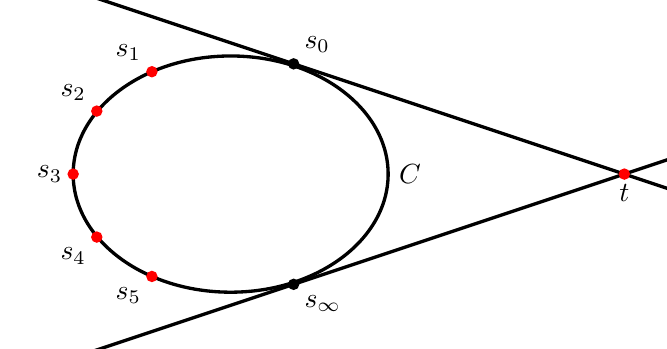
\begin{tikzpicture}[very thick]
  \draw (0,0) ellipse (2 and 1.5) (2,0) node [right] {$C$};
  \draw[shorten >=-3cm, shorten <=-3cm] (0.8, 1.4) -- (5,0);
  \draw[shorten >=-3cm, shorten <=-3cm] (0.8, -1.4) -- (5,0);

  \draw[red, fill] (5,0) circle (0.05) node [black, below] {$t$};
  \draw[fill] (0.8, 1.4) circle (0.05) node [above right] {$s_0$};
  \draw[fill] (0.8, -1.4) circle (0.05) node [below right] {$s_\infty$};

  \draw[red, fill]
  (-1, 1.3) circle (0.05) node [black, above left] {$s_1$}
  (-1.7, 0.8) circle (0.05) node [black, above left] {$s_2$}
  (-2, 0) circle (0.05) node [black, left] {$s_3$}
  (-1, -1.3) circle (0.05) node [black, below left] {$s_5$}
  (-1.7, -0.8) circle (0.05) node [black, below left] {$s_4$};
\end{tikzpicture}

%%% Local Variables:
%%% mode: latex
%%% TeX-master: "../main"
%%% End:
